\documentclass[a4paper,11pt,titlepage,french]{article}
% classe de document pour LaTeX qui définit les paramètres généraux du document : 
    % a4paper : définit le format de papier sur lequel le document doit être imprimé (a4paper format standard)
    % 11pt : définit la taille de police de base à 11 points
    % titlepage : demande à LaTeX d'insérer une page de titre dans le document
    % french : Cette option indique à LaTeX que le document est rédigé en français
% TODO : \input{chemin vers le fichier de setup} 
    % le fichier de setup devra contenir l'ensemble des usepackage suivants et les variables globales
% ----------------
% LIBRAIRIES LATEX
% ----------------
\usepackage[main=french]{babel}
\usepackage[T1]{fontenc}
\usepackage{fontspec}
\usepackage{fancyhdr}
\usepackage{xspace, graphicx}
\usepackage{longtable}
\usepackage[table]{xcolor}
\usepackage{hyperref}
\usepackage{enumitem}	
\usepackage{listings}
\usepackage{tcolorbox}
\usepackage{color}
\usepackage{courier}

% To use animUML example.tex file
\usepackage[T1]{fontenc}
\usepackage{graphicx}
\usepackage[export]{adjustbox}
\usepackage{float}

\usepackage{caption}
\usepackage{lastpage}

% ------------------
% VARIABLES GLOBALES
% ------------------
\newcommand{\version}{0.1}
\newcommand{\revision}{0}
\newcommand{\documentName}{Manuel d'utilisation}
\newcommand{\documentNameAbrev}{INST}
\newcommand{\prose}{ProSE}
\newcommand{\creator}{Paul TREMOUREUX}
\newcommand{\projectName}{Passerelle Android-CAN vers banc CAN réel ou simulé}
\newcommand{\annee}{2024}
\newcommand{\teamName}{CANvengers} 
\newcommand{\teamNumber}{B1}
\newcommand{\client}{KEREVAL}
\newcommand{\nomLogiciel}{CANgateway} 
\newcommand{\nomApplication}{CANdroid} 

\setcounter{secnumdepth}{4} % Pour avoir une numérotation jusqu'au niveau 4
\renewcommand{\theparagraph}{\thesubsubsection.\arabic{paragraph}} % Pour numéroter les paragraphes à partir du niveau 3
\makeatletter % Redéfinit la commande \paragraph pour qu'elle utilise les paramètres de formatage de la commande \subsubsection.
\renewcommand\paragraph{\@startsection{paragraph}{4}{\z@}%
    {-3.25ex \@plus -1ex \@minus -.2ex}%
    {1.5ex \@plus .2ex}%
    {\normalfont\normalsize\bfseries}}
\makeatother
\setlength{\parindent}{0pt} % Supprime l'indentation par défaut

% -------------------------------------------------------
% --------------------------
% PARAMETRES HEADER / FOOTER 
% --------------------------
\pagestyle{fancy} % permet de personnaliser l'apparence de l'en-tête et du pied de page de chaque page du document
\setlength{\hoffset}{-40pt} % définis la marge horizontale gauche
\setlength{\topmargin}{-25pt} % définis la marge supérieure 
\setlength{\headsep}{10pt} % définis l'espace vertical entre l'en-tête et le corps de texte 
\renewcommand{\headheight}{60pt} % redéfinis la hauteur de l'en-tête
\renewcommand{\headwidth}{450pt} %  redéfinis la largeur de l'en-tête
\setlength{\textwidth}{450pt} % définis la largeur du corps de texte
\setlength{\textheight}{604pt} %  définis la hauteur du corps de texte
\renewcommand{\footrulewidth}{0.1mm} % redéfinis la largeur de la ligne de séparation de pied de page
\fancyhf{} % vide les entêtes et pieds de page précédemment définis
    % HEADER %
    \fancyhead[LO]{\bf \includegraphics[width=80pt]{../figures/eseo.png}\\ % fancyhead - personnaliser l'en-tête avec 2 arguments : orientation "LO" pour "Left Odd" / contenu "\bf" pour texte en gras + "\includegraphics" inclure le logo de l'ESEO
        \medskip % ajoute espace vertical moyen (≃ 6 points)
        {\prose} équipe {\teamNumber} {\annee}} % texte en dessous de l'image de la partie gauche du pdf
    \fancyhead[RO]{\bf 
\includegraphics[width=90pt]{../figures/logo_kereval.png}\\ % fancyhead - personnaliser l'en-tête avec 2 arguments : orientation "RO" pour "Right Odd" / contenu "\bf" pour texte en gras + "\includegraphics" inclure le logo de l'entreprise
        {\small{Ref. {\documentNameAbrev}\_{\teamNumber}}}} % texte en dessous de l'image de la partie droite du pdf
    % FOOTER %
    \fancyfoot[LO]{\sl {\it Version {\version} - Révision {\revision}}} % fancyfoot - personnaliser le pied de page avec 2 arguments : position "LO" pour "Left Odd" / contenu "\sl" + "\it" pour texte en italique de la version et la révision
    \cfoot{\copyright {\annee} Droits réservés {\teamName}} % insérer texte au centre du pied de page
    \fancyfoot[RO]{\thepage/\pageref{LastPage}} % pied de page partie droite : numéro de page
% ------------------------------
% FIN PARAMETRES HEADER / FOOTER 
% ------------------------------
\definecolor{darkWhite}{rgb}{0.90,0.90,0.90}

\lstset{
    backgroundcolor=\color{darkWhite},
    breakatwhitespace=false,
    breaklines=true,
    commentstyle=\color{red},
    deletekeywords={...},
    escapeinside={\%*}{*)},
    keywordstyle=\color{blue},
    language=bash,
    stepnumber=0,
    stringstyle=\color{orange},
    tabsize=4,
    columns=fullflexible, 
    title=\lstname,
}

\lstdefinestyle{frameStyle}{
    basicstyle=\footnotesize,
    numbers=left,
    numberstyle=\tiny\color{black}
}
 
\tcbuselibrary{listings,skins,breakable}
 
\newtcblisting{customFrame}{
    width=\textwidth,
    listing only,
    listing options={style=frameStyle}
}

% --------------
% DEBUT DOCUMENT 
% --------------
\begin{document}
\sloppy % relâche les règles de justification de texte pour éviter des espaces trop larges
\renewcommand{\arraystretch}{1.3} % augmente la hauteur des lignes d'un tableau

%-----------------------------------------------
%   The titles of the parts
%-----------------------------------------------
\makeatletter
% Adds a sub-subparagraph level
\newcounter{subsubparagraph}[subparagraph]
\renewcommand\thesubsubparagraph{%
    \thesubparagraph.\@arabic\c@subsubparagraph}
\newcommand\subsubparagraph{%
    \@startsection{subsubparagraph}               % counter
    {6}                                           % level
    {0em}                                         % indentation
    {1em}                                         % before the title
    {1em}                                         % after the title
    {\normalsize\hspace{6em}\color{colorTitle}} % style (overloaded by the title format)
}
\newcommand\l@subsubparagraph{\@dottedtocline{6}{13em}{6em}}
\newcommand{\subsubparagraphmark}[1]{}
\providecommand*{\toclevel@subsubparagraph}{6}

\setcounter{tocdepth}{6}    % Allows the paragraph in the table of contents
\setcounter{secnumdepth}{6} % Allows the numbering of the sub-paragraph

\makeatother
% -------------------
% PAGE DE GARDE {p.1}
% -------------------
\begin{center} % centre le contenu de la commande
    \vspace*{2cm} % ajout d'espace
    \rule[0.5ex]{0.7\textwidth}{0.1mm}\\ % ajout ligne horizontale : décalage verticale "ex" / largeur de page "%" / épaisseur "mm"
    \vspace*{2mm} % ajout d'espace
        {\Huge {\textsc{\bf {\documentName}}}} % crée un titre : police en gras "\bf" / petites capitales "\textsc" / grande taille polile "\Huge" 
    \vspace{0.4cm}\\ % ajout d'espace / "\\" : retour à la ligne 
        {\large\bf {\prose} {\teamNumber} {\annee} - {\teamName}}\\ % crée un titre : police en gras "\bf" / taille de police relativement grande "\large"
    \vspace*{1mm}
        {\large\bf {\projectName}}\\ % crée un titre 
    \rule[0.5ex]{0.75\textwidth}{0.1mm}\\ % ajout ligne horizontale
    \vspace{2cm} 
    \begin{tabular}{|c|c|} % crée un tableau avec 2 colonnes 
        \hline % crée une ligne dans le tableau // & : séparateur colonne
            Responsable du document & {\creator}                      \\
            État du document        & En révision                     \\
            Version                 & {\version}                      \\
            Révision                & {\revision}                     \\
        \hline
    \end{tabular}
\end{center}
\vspace{3cm} 
% -----------------------
% FIN PAGE DE GARDE {p.1}
% -----------------------
 
% ---------------------
% TABLEAU VERSION {p.2}
% ---------------------
% \noindent % Modifie l'espacement horizontal entre les colonnes
%
% Tableau des version à remplir à chaque fois que vous apportez une modification
%
\newpage % nouvelle page 
\begin{center}
\begin{longtable}[l]{|p{2cm}|p{5.8cm}|p{2.8cm}|p{1.4cm}|p{1.7cm}|}
    \hline
        \textbf{Date} & \textbf{Actions} & \textbf{Auteur} & \textbf{Version} & \textbf{Révision}\\
    \hline
        05/04/2023 & Création du document & Elisa\newline Declerck & 0.0 & 0\\
    \hline
        03/04/2023 & Réalisation du diagramme de séquence de "Démarrer le SàE" & Paul\newline  TRÉMOUREUX & 0.0 & 1 \\
    \hline
        07/04/2023 & Rédaction de Portée & Gabriel\newline MARQUETTE & 0.0 & 2\\
    \hline
        07/04/2023 & Rédaction de Objet & Gabriel\newline  MARQUETTE	& 0.0 & 3 \\
    \hline
        08/04/2023 & Réalisation de certains diagrammes de séquence & Théo\newline  BÉNARD & 0.0 & 4 \\	
    \hline
        10/04/2023 & Correction des diagrammes de séquence & Elisa\newline  DECLERCK & 0.0 & 5 \\	
    \hline
        12/04/2023 & Rédaction de la machine à états de Sender & Gabriel\newline  MARQUETTE & 0.0 & 6\\
    \hline
        12/04/2023 & Rédaction des descriptions des classes Sender, Basket et Network & Gabriel\newline  MARQUETTE & 0.0 & 7\\
    \hline
        12/04/2023 & Rédaction de la description générale des classes suivante : GUI, UI, Dealer, Logger, Object, Frame, Sniffer & Paul\newline  TRÉMOUREUX & 0.0 & 8\\
    \hline
        12/04/2023 & Rédaction de diagrammes de séquence & Thomas\newline  ROCHER & 0.0 & 9\\
    \hline
        12/04/2023 & Rédaction de diagrammes de séquence & Camille\newline  LENNE & 0.0 & 10\\
    \hline
        13/04/2023 & Correction du CU "Démarrer le SàE" & Paul\newline  TRÉMOUREUX & 0.0 & 11\\
    \hline
        13/04/2023 & Relecture et correction des doublons de descriptions générales de toutes les classes & Paul\newline  TRÉMOUREUX & 0.1 & 0\\
    \hline
        13/04/2023 & Rédaction de la description de l'architecture candidate & Elisa\newline  DECLERCK & 0.1 & 1\\
    \hline
	    13/04/2023 & Ajout des multiplicitées au diagramme de classe & Elisa\newline  DECLERCK & 0.1 & 2\\
    \hline
        15/04/2023 & Relecture des parties Références, Types de données et Services Offerts & Camille\newline LENNE & 0.1 & 3 \\
    \hline
        15/04/2023 & Relecture et correction de la description des diagrammes de séquence & Camille \newline LENNE & 0.1 & 4\\
    \hline
        16/04/2023 & Correction CU Reconnecter l'application {\nomApplication} & Thomas\newline  ROCHER & 0.1 & 5\\
    \hline
        16/04/2023 & Correction de la description de l'architecture candidate & Thomas\newline  ROCHER & 0.1 & 6\\
    \hline
        16/04/2023 & Inclusion de la MAE de GUI	& Elisa\newline  DECLERCK & 0.1 & 7 \\
    \hline
        17/04/2023 & Relecture section 2.2 + rédaction de note & Thomas\newline  ROCHER & 0.2 & 0\\		
    \hline
        17/04/2023 & Relecture partie + rédaction de note & Gabriel\newline  MARQUETTE & 0.2 & 1\\
    \hline
        17/04/2023 & Rédaction de la description de la MAE & Elisa\newline  DECLERCK & 0.2 & 2\\
    \hline
        18/04/2023 & Correction du schéma et de la description de la MAE de GUI & Elisa\newline  DECLERCK & 0.2 & 3\\
    \hline
        18/04/2023 & Correction de la section 2.2 & Thomas\newline  ROCHER & 0.2 & 4\\
    \hline
        19/04/2023 & Correction du dossier dans sa globalité & Théo\newline  BÉNARD & 1.0 & 0\\
    \hline
        26/04/2023 & Correction de certaines descriptions des diagrammes de séquence & Elisa\newline  DECLERCK & 1.0 & 1\\
    \hline
        27/04/2023 & Création de la MAE de UI et rédaction de sa description & Elisa\newline  DECLERCK & 1.0 & 2\\
    \hline
        27/04/2023 & Correction de la MAE de GUI & Gabriel\newline  MARQUETTE & 1.0 & 3\\
    \hline
        27/04/2023 & Correction de l'ensemble du dossier à la suite de l'audit consultatif & Elisa\newline  DECLERCK & 1.0 & 3\\
    \hline
        30/04/2023 & Relecture de la partie CANgateway de la conception détaillée & Thomas\newline  ROCHER & 1.1 & 0\\
    \hline
        24/05/2023 & Ajout de l'architecture du programme {\nomLogiciel} & Elisa\newline  DECLERCK & 1.1 & 1\\
    \hline
        26/05/2023 & Correction de la MAE de GUI & Elisa \newline DECLERCK & 1.1 & 2\\
    \hline
        26/05/2023 & Rédaction de la description des classes du programme {\nomLogiciel} & Elisa \newline DECLERCK & 1.1 & 3\\
    \hline
        28/05/2023 & Rédaction de la description des classes proxyGUI, proxyLogger, Dispatcher et Postman du programme {\nomLogiciel} & Thomas \newline ROCHER & 1.1 & 4\\
    \hline
        30/05/2023 & Rédaction des différents diagrammes de classes & Gabriel \newline MARQUETTE & 1.1 & 5 \\    
    \hline
        30/05/2023 & Rédaction du protocole de communication & Thomas \newline ROCHER & 1.1 & 6 \\    
    \hline
        31/05/2023 & Relecture de la conception détaillée & Thomas \newline ROCHER & 1.2 & 0 \\    
    \hline
        05/06/2023 & Correction dossier de conception & Elisa \newline DECLERCK & 1.2 & 1 \\
    \hline
        05/06/2023 & Correction et relecture de la conception détaillée coté Android & Camille \newline LENNE & 1.2 & 2 \\
    \hline
        09/06/2023 & Correction du dossier après audit normatif de code & Elisa \newline DECLERCK & 1.2 & 3 \\
    \hline
        13/06/2023 & Correction du dossier de conception dans sa globalité & Thomas \newline ROCHER & 2.0 & 0 \\
    \hline

\end{longtable}

\captionof{table}{Table des évolutions et validations internes du document}
\end{center}
\newpage % nouvelle page 
% -------------------------
% FIN TABLEAU VERSION {p.2}
% -------------------------

% --------------
% SOMMAIRE {p.3}
% --------------
\tableofcontents % génére table des matières en fonction des commandes "\section{}"
% ------------------
% FIN SOMMAIRE {p.3}
% ------------------

% ---------------
% BUT DU DOCUMENT
% ---------------
% Auteurs : Camille Constant, Paul Trémoureux

\section{Introduction}
\label{sec:intro}

\subsection{Contexte}
\label{sec:intro:contexte}

\noindent\begin{tabularx}{\linewidth}{|p{3.5cm}|X|}
\hline
{\bf Produit à tester :} & {\projet} - version {\versionProjet}\\
\hline
{\bf Type de produit :} & {\produit}.\\
\hline
{\bf Commanditaire :} & {\client}\\
\hline
{\bf Développeur :} & {\equipe}\\
\hline
{\bf Testeur :} & {\equipe}\\
\hline
\end{tabularx}

\subsection{Objet}
\label{sec:intro:objet}

Ce document décrit l'activité de test système qui sera menée par {\equipe} durant le projet {\projet} dans le but de valider le produit suivant : {\produit}. Il est rédigé sous la responsabilité du Responsable Qualité-Test (RQT), sous la direction du Chef de Projet (CdP), conformément au Plan d'Assurance Qualité Logicielle (PAQL) élaboré sous la responsabilité du RQT (cf. section~\ref{sec:eqTest}, Équipe de test).

\subsection{Portée} 
\label{sec:intro:portee}

Sont concernés par ce document :
\begin{itemize}
    \item les testeurs : afin que ceux-ci connaissent le périmètre des tests (ce qu'ils vont tester), l'environnement de test (comment les tests seront mis en {\oe}uvre) et le processus de test (comment s'y prendre et rendre compte des résultats lors de l'exécution des tests) ;
    \item les développeurs : à titre informatif, afin que ceux-ci sachent comment va être validée leur production ; à titre indicatif afin qu'ils sachent, par la description de la gestion des anomalies, comment ils s'interfaceront avec l'équipe de test ;
    \item le client : ce plan de test fait l'objet d'une contractualisation avec le client pour déterminer le périmètre des tests menés pour valider le produit livré et les niveaux d'acceptation de cette validation ;
    \item les auditeurs : ce plan de test, ainsi que son implication, feront l'objet d'audits par la société Formato.
\end{itemize}

\subsection{Copyright}
\label{sec:intro:copyright}
Cf. {\refPAQL} (section 1.3. Copyright).

\subsection{Présentation du système} 
\label{sec:intro:scope}

Le système développé est un ensemble de 2 programmes : une application Android nommé {\appliA} déployé sur un smartphone Android et un programme C nommé {\appliC} déployé sur une Raspberry Pi.
L'application {\appliA} sera relié au programme {\appliC} par un réseau TCP/IP. La Raspberry Pi sera connectée à un réseau CAN pour dialoguer avec Tableau de Bord (soit banc de test physique soit simulateur sur un PC).
Ce projet permettra d'envoyer des trames depuis l'application {\appliA} vers Tableau de Bord afin de piloter ce dernier à distance.

\subsection{Références}
\label{sec:intro:ref}

\subsubsection{Documents de référence internes}
\noindent\begin{tabularx}{\linewidth}{|p{3cm}|X|p{1.4cm}|X|}
\hline
\textbf{Ref.} & \textbf{Nom et auteur} & \textbf{Version} & \textbf{Source}\\
\hline
{\refSpec} & Dossier de spécifications - \newline {\equipe} & 2.0.0 & se2024-b1.doc/specification/livrables\\
\hline
%Si client impliqué dans le PAQL
{\refPAQL} & Plan d'Assurance Qualité Logiciel - {\rqt} & 1.0.0 & pdf sur le dépôt\\
\hline
\end{tabularx}

\subsubsection{Documents de référence externes}
\noindent\begin{tabularx}{\linewidth}{|p{2.8cm}|X|}
\hline
\textbf{Ref.} & \textbf{Nom} \\
\hline
[ISO-829-2008] & Documentation de test logiciel\\
\hline
[ISO/IEC/IEEE 29119-1:2022] & Ingénierie du logiciel et des systèmes - Essais du logiciel - Partie 1: Concepts généraux\\
\hline
\end{tabularx}

\subsection{Glossaire et abréviations}
\label{sec:intro:termes}

Ce sont les termes et abréviations nécessaires à la compréhension de l'activité de test (les termes techniques propres au projet seront indiqués dans le dossier de spécification).

\subsubsection{Abréviations}

\noindent\begin{longtable}[c]{|p{.20\textwidth}|p{.80\textwidth}|}
\hline
CdP & Chef de Projet\\
\hline
IHM & Interface Homme-Machine\\
\hline
PAQL & Plan Assurance Qualité Logicielle\\
\hline
RQT & Responsable Qualité et Test\\
\hline
\end{longtable}

\subsubsection{Glossaire}

\noindent\begin{longtable}[c]{|p{.20\textwidth}|p{.80\textwidth}|}
\hline
{\bf Campagne de test} & Activité qui consiste à dérouler un ensemble de jeux de test. Un dossier de test est produit à l'issue d'une campagne.\\
\hline
{\bf Cas de test} & Déclinaison d'un test précisant les valeurs utilisées pour les variables du test ainsi que les résultats attendus.\\
\hline
{\bf Dossier de test} & Ensemble documentaire qui contient la description des scénarios et des cas de tests, ainsi que l'exécution des jeux de test. Le dossier de test est le reflet d'une campagne de test. \\
\hline
{\bf Jeux de test} & Ensemble des scénarios et cas de tests permettant de tester un produit logiciel. L'enchaînement des cas et scénarios de tests est relatif à une stratégie de test précisée dans le plan de test.\\
\hline
{\bf Plan de test} & Document décrivant le déroulement d'un jeu de test : stratégie de test, critères d'arrêt, planification.\\
\hline
{\bf Scénarios de test} & Ensemble de cas de tests cohérents permettant de traiter un objectif fonctionnel.\\
\hline
{\bf Test d'intégration} & Vérification effectuée pour montrer des défauts dans les interfaces et interactions de composants ou systèmes intégrés.\\
\hline
{\bf Test de non régression} & Vérification qu'une nouvelle version du produit fonctionne sans dégradation (technique, fonctionnelle, performance) par rapport à la version précédente.\\
\hline
{\bf Test de validation} & Vérification que le produit est cohérent et complet par rapport aux spécifications fonctionnelles.\\
\hline
{\bf Test fonctionnel} & Test (vu de l'utilisateur) du bon fonctionnement d'un produit logiciel, d'une fonctionnalité ou d'une fonction de base. Vérification par rapport aux spécifications.\\
\hline
{\bf Test système} & Vérification que le système dans son ensemble est cohérent et complet par rapport aux spécifications fonctionnelles et techniques.\\
\hline
{\bf Test unitaire} & Vérification que les composants logiciels individuels sont cohérents et complets par rapport aux spécifications.\\
\hline
\end{longtable}

Voir également le \href{https://www.cftl.fr/wp-content/uploads/2018/10/Glossaire-des-tests-logiciels-v3_2F-ISTQB-CFTL-1.pdf}{[Glossaire CFTL/ISTQB des termes utilisés en tests de logiciels]}.\\

\subsection{Conformité}
\label{sec:intro:conf}

Ce plan de test est conforme aux normes~:

\begin{itemize}
    \item IEEE Std. 1012-1986
    \item ISO Std. 829-2008
    \item IEEE Std. 1008-1987
    \item ISO/IEC/IEEE 29119-1:2022
\end{itemize}
% -------------------------------
% UTILISATION CANdroid/CANgateway
% -------------------------------
%
% Comment utiliser l'application ?
%
\newpage % nouvelle page
\section{Utilisation de {\nomApplication}/{\nomLogiciel}}

\subsection{Matériel nécessaire}
L'utilisation de l'application {\nomApplication} et du programme {\nomLogiciel} nécessite un matériel spécifique. Ce matériel a été défini avec le client et a été validé via tests. CANvengers ne garantit pas le bon fonctionnement du projet {\guillemetleft} {\projectName} {\guillemetright}. Le matériel testé est le suivant :
\begin{itemize}
    \item Banc de Test : KERAVAL Banc de Test ;
    \item Ordinateur : Linux Ubuntu (64-bit) ;
    \item Passerelle Raspberry-CAN : PEAK PCAN;USB IPEH-002021 175459 ;
    \item Passerelle Tableau de Bord-CAN : RS485/CAN HAT;
    \item Raspberry : pi 3B+ ;
    \item Smartphone : Samsung Galaxy A20e sous système Android 9.
\end{itemize}

\subsection{Logiciels nécessaires}
L'utilisation du système développé dans ce projet nécessite l'installation de certains logiciels :
\begin{itemize}
    \item Application {\nomApplication} : version 2.0.0 ;
    \item Programme {\nomLogiciel} : version 2.0.0 ;
    \item \hyperref[ICSim]{Simulateur ICSim} : version du 12/06/2020.
\end{itemize}
Pour installer ces logiciels veuillez suivre les instructions du \hyperref[INST]{Manuel\_Installation\_SANS\_B1\_2024}.\\

\subsection{Préparation}
En fonction de l'utilisation souhaitée, Utilisateur peut n'avoir besoin que d'une partie du matériel.

\subsubsection{Application {\nomApplication} seule}
Pour une utilisation de l'application {\nomApplication} seule, les éléments suivants sont nécessaires :
\begin{itemize}
    \item Application {\nomApplication} ;
    \item Smartphone.
\end{itemize}

\subsubsection{Utilisation de la Raspberry Pi}
Pour une utilisation de l'application {\nomApplication} avec la Raspberry Pi, les éléments suivant sont nécessaires :
\begin{itemize}
    \item Application {\nomApplication} ;
    \item Programme {\nomLogiciel} ;
    \item Raspberry ;
    \item Smartphone.
\end{itemize}

\subsubsection{Utilisation du Simulateur ICSim}
Pour une utilisation de l'application {\nomApplication} avec la Raspberry Pi et le Simulateur ICSim, les éléments suivant sont nécessaires :
\begin{itemize}
    \item Application {\nomApplication} ;
    \item Ordinateur ;
    \item Passerelle Raspberry-CAN ;
    \item Passerelle Tableau de Bord-CAN ;
    \item Programme {\nomLogiciel} ;
    \item Raspberry ;
    \item Simulateur ICSim ;
    \item Smartphone.
\end{itemize}

\subsubsection{Utilisation du Banc de Test}
Pour une utilisation de l'application {\nomApplication} avec la Raspberry Pi, les éléments suivant sont nécessaires :
\begin{itemize}
    \item Application {\nomApplication} ;
    \item Banc de Test ;
    \item Passerelle Tableau de Bord-CAN ;
    \item Programme {\nomLogiciel} ;
    \item Raspberry Pi ;
    \item Smartphone.
\end{itemize}

\subsubsection{Utilisation du Simulateur ICSim et du Banc de Test}
Pour une utilisation de l'application {\nomApplication} avec la Raspberry Pi, les éléments suivant sont nécessaires :
\begin{itemize}
    \item Application {\nomApplication} ;
    \item Banc de Test ;
    \item Ordinateur ;
    \item Passerelle Raspberry-CAN ;
    \item Passerelle Tableau de Bord-CAN ;
    \item Programme {\nomLogiciel} ;
    \item Raspberry Pi ;
    \item Simulateur ICSim ;
    \item Smartphone.
\end{itemize}

\subsubsection{Tests}
Pour l'exécution des tests, les logiciels suivants sont nécessaires :
\begin{itemize}
    \item Tests du programme {\nomLogiciel} :
    \begin{itemize}
        \item GNU Compiler Collection : Logiciel utilisé pour compiler les tests ;
        \item CMocka : Module de tests (notamment utilisé pour les tests unitaires) ;
        \item Apache JMeter : Logiciel utilisé pour les tests de serveurs.
    \end{itemize}
    \item Tests de l'application {\nomApplication} :
    \begin{itemize}
        \item JUnit : Logiciel utilisé pour les tests unitaires ;
        \item Robot Framework : Logiciel utilisé pour les tests de validation.
    \end{itemize}
\end{itemize}

\subsection{Branchement}
Pour l'utilisation du matériel veuillez suivre le branchement décrit ci-dessous selon votre utilisation.

\subsubsection{Simulateur ICSim}

Pour utiliser le Simulateur ICSim avec notre système, il faut pouvoir connecter votre PC avec la Raspberry Pi. Pour cela, vous pouvez utiliser le PCAN-USB de PEAK. Connectez la partie USB à votre PC et la partie CAN à la Raspberry Pi.\\

Voici le lien du site de PCAN-USB : \href{https://www.peak-system.com/PCAN-USB.199.0.html?&L=2}{Interface CAN pour USB}.\\

Il y a 3 pins importantes sur les 9 pins du connecteur CAN :
\begin{itemize}
    \item CAN\_L : pin 2 ;
    \item CAN\_H : pin 7 ;
    \item GND : pin 6.
\end{itemize}

\begin{minipage}
    \textwidth
    \centering
    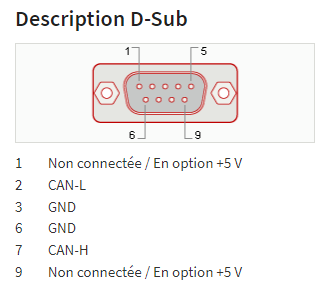
\includegraphics[width=0.5\textwidth]{../figures/D-Sub_PEAK.png}
    \captionof{figure}{Description des pins du PCAN-USB}
\end{minipage}

Pour connecter ses pins à la Raspberry Pi, vous pouvez utiliser un connecteur connecteur DB9 femelle et souder des fils sur les pins 2, 7 et 6.\\

Connectez ensuite les fils CAN\_H et CAN\_L aux pins du RS485 CAN HAT et GND à une pin GND de la Raspberry Pi.\\

Attention, pour utiliser ICSim, il vous faut utiliser un RS485 CAN HAT dont la résistance de terminaison est soudée.\\

\subsubsection{Banc de Test}

Pour utiliser le Banc de Test, vous n'avez pas besoin d'un connecteur DB9 supplémentaire, celui-ci est déjà présent sur le Banc de Test.\\

Trouvez le connecteur DB9 dans le Banc de Test, de la même manière que pour le connecteur DB9 précédent, les pins 2 et 7 sont soudées à des fils que vous pouvez directement connecter au RS485 CAN HAT.\\

Attention cependant, pour utiliser le Banc de Test, il vous faut utiliser un RS485 CAN HAT dont la résistance de terminaison est désoudée.\\

\subsubsection{Banc de Test et Simulateur ICSim}

Pour utiliser à la fois le Banc de Test et le simulateur ICSim, il vous suffit de connecter le connecteur DB9 du Banc de Test au PCAN-USB que vous reliez à votre PC. Reliez également les pins 2 et 7 du Banc de Test au RS485 CAN HAT.\\

De la même manière que pour les deux autres utilisations, vous devez utiliser un RS485 CAN HAT dont la résistance de terminaison est désoudée.\\

\subsection{Démarrage}

Afin que le système fonctionne au mieux, nous vous proposons de suivre les étapes suivantes dans l'ordre indiqué.

\subsubsection{Banc de Test}

Dans le cadre de notre projet, nous tenons à préciser que nous n'avons pas utilisé le Banc de Test, mais uniquement le simulateur ICSim. Par conséquent, nous ne disposons pas des informations nécessaires pour décrire en détail le cycle d'allumage du dispositif. Notre travail s'est principalement concentré sur l'utilisation du simulateur et la mise en œuvre des fonctionnalités requises.

\subsubsection{Simulateur ICSim}

Si vous souhaitez utiliser le Simulateur ICSim, commencez pas brancher le PCAN-USB à votre PC et à la Raspberry Pi.\\
Si vous le branchez sur un OS Linux, vous n'avez rien à faire, le driver permettant d'utiliser le PCAN-USB est déjà installé sur le noyau Linux.\\
Sinon, vous avez besoin de télécharger le driver sur le site de PEAK : \href{https://www.peak-system.com/PCAN-USB.199.0.html?&L=2}{Support PEAK}.\\
Si le PCAN-USB est branché et que le driver est installé, la LED rouge du PCAN-USB doit être allumée.\\

Commencez par activer le CAN sur votre ordinateur : 
\begin{itemize}
    \item Dans un terminal, tapez :
\vspace{-1.8\baselineskip} 
\begin{lstlisting}
    sudo ip link set can0 down
    sudo ip link set can0 type can bitrate 125000
    sudo ip link set can0 up
\end{lstlisting}
    \item Vérifiez que le CAN est bien activé :
\vspace{-1.8\baselineskip} 
\begin{lstlisting}
    sudo ip -details link show can0
\end{lstlisting}
Vous devriez voir ceci : 
\vspace{-1.8\baselineskip}
\begin{lstlisting}
    3: can0: <NOARP,UP,LOWER_UP,ECHO> mtu 16 qdisc pfifo_fast state UP mode DEFAULT group default qlen 10
    link/can  promiscuity 0 minmtu 0 maxmtu 0 
    can state ERROR-ACTIVE (berr-counter tx 0 rx 95) restart-ms 0 
	  bitrate 125000 sample-point 0.875 
	  tq 500 prop-seg 6 phase-seg1 7 phase-seg2 2 sjw 1
	  pcan_usb: tseg1 1..16 tseg2 1..8 sjw 1..4 brp 1..64 brp-inc 1
	  clock 8000000 numtxqueues 1 numrxqueues 1 gso_max_size 65536 gso_max_segs 65535 parentbus usb parentdev 2-2.1:1.0 
\end{lstlisting}
\end{itemize}

Pour rappel, le bus CAN est fonctionnel quand il est dans l'état ERROR-ACTIVE. Dans l'état STOPPED, il n'a pas démarré. Dans l'état ERROR-PASSIVE, il est en erreur et il faut le redémarrer pour qu'il fonctionne à nouveau.\\

Lorsque le bus CAN est fonctionnel, la LED rouge du PCAN-USB clignote lentement (elle cligonte rapidement lorsque des trames sont émises).\\

Dès que le bus CAN est fonctionnel, vous pouvez lancer le Simulateur ICSim :
\begin{enumerate}
    \item Ouvrez un terminal et placez vous dans le dossier ICSim ;
    \item Tapez :
\vspace{-1.8\baselineskip}
\begin{lstlisting}
    ./icsim can0
\end{lstlisting}
    \item Ouvrez un second terminal et placez vous dans le dossier ICSim ;
    \item Tapez :
\vspace{-1.8\baselineskip}
\begin{lstlisting}
    ./controls can0
\end{lstlisting}
\end{enumerate}

Cela est sensé vous ouvrir deux fenêtres, une pour le Simulateur ICSim et une pour le contrôleur : 

\begin{minipage}
    \textwidth
    \centering
    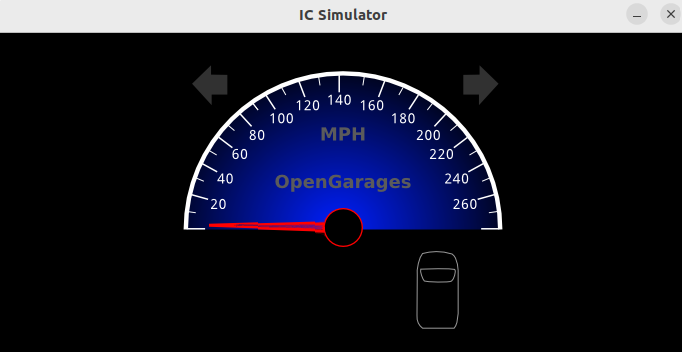
\includegraphics[width=0.80\textwidth]{../figures/ICSIM.png}
    \captionof{figure}{ICSim}
    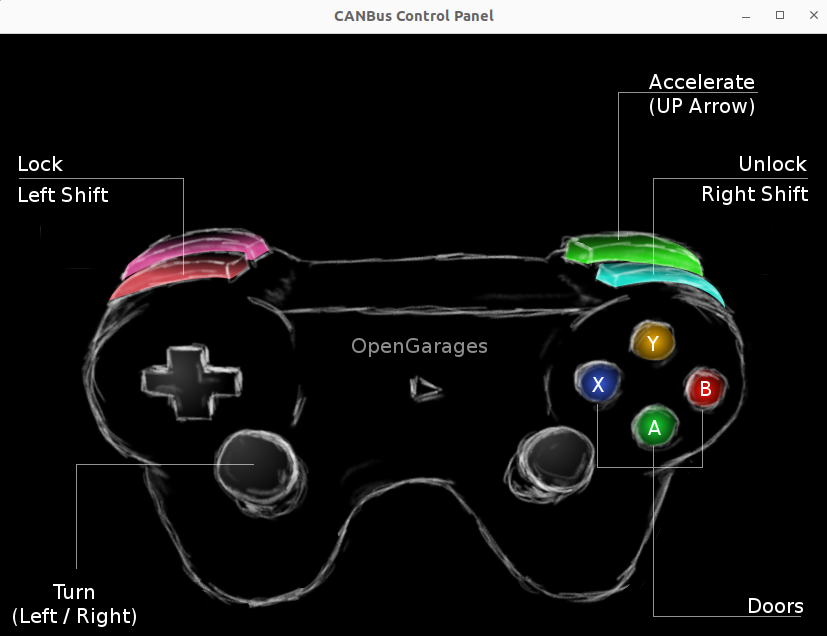
\includegraphics[width=\textwidth]{../figures/CONTROLEUR.png}
    \captionof{figure}{Contrôleur}
\end{minipage}

le Simulateur ICSim est démarré, vous pouvez voir toutes les trames émises entre le simulateur et le contrôleur grâce aux commandes suivantes :
\begin{itemize}
    \item Permet d'afficher toutes les trames sniffées :
\vspace{-1.8\baselineskip}
\begin{lstlisting}
    candump can0
\end{lstlisting}
    \item Permet de n'afficher que les nouvelles trames sniffées (évite d'afficher les même trames à répétition) :
\vspace{-1.8\baselineskip}
\begin{lstlisting}
    cansniffer -c can0
\end{lstlisting}
\end{itemize}

\subsubsection{Programme {\nomLogiciel}}

Pour utiliser le programme {\nomLogiciel}, commencez par vous connecter à la Raspberry Pi via SSH, ou, si vous préférez, connectez un écran et un clavier à la Raspberry Pi.\\

Ouvrez un terminal de la Raspberry Pi et placez vous dans le dossier /home/pi. \\

Vérifiez que le programme {\nomLogiciel} est bien présent dans le dossier, sinon, veuillez lire le \hyperref[INST]{Manuel\_Installation\_SANS\_B1\_2024}, dans la section "Installation du programme {\nomLogiciel}".\\

Pour lancer le programme {\nomLogiciel}, tapez :
\vspace{-1.8\baselineskip}
\begin{lstlisting}
    sudo ./CANgateway.out
\end{lstlisting}
(Entrez le mot de passe si nécessaire)\\

Lorsque le programme est lancé, vous pouvez voir le message suivant s'afficher dans la console :
\vspace{-2.5\baselineskip}
\begin{lstlisting}
    Lancement du programme
\end{lstlisting}

\subsubsection{Application {\nomApplication}}
Si l'application {\nomApplication} est installée sur le Smartphone, cliquer sur l'icone de l'application {\nomApplication} sur l'écran.

Si l'application {\nomApplication} n'est pas installée sur le Smartphone, suivre le \hyperref[INST]{Manuel\_Installation\_SANS\_B1\_2024}.

\subsection{Manipulation}
Lors de votre utilisation du projet, seuls les fonctionnalités décrites dans \hyperref[SPEC]{dossier\_de\_specifi-cation\_SPEC\_B1\_2024} et \hyperref[plan_de_test]{plan\_de\_test \_TEST\_B1\_2024}. Toute utilisation de l'application {\nomApplication} et du programme {\nomLogiciel} sortant de ce cadre peut amener à des disfonctionnements dont l'équipe {\teamName} n'est pas responsable.

\subsubsection{Application {\nomApplication}}
Durant l'utilisation normale du projet, plusieurs interactions entre Utilisateur et l'application {\nomApplication} sont prévues. Ces interactions sont les suivantes :

\begin{itemize}
    \item Partie haute de l'écran
    \begin{itemize}
        \item Ajout de trame
        \item Ajout d'objet
        \item Défilement
        \item Déroulement des menu d'objet
        \item Mise en marche/arrêt de l'envoi de trames
        \item Reconnexion
        \item Séléctions d'éléments
        \item Suppression d'éléments
    \end{itemize}
    \item Partie basse de l'écran
    \begin{itemize}
        \item Défilement
        \item Enregistrement du sniffer
        \item Mise en marche/arrêt du sniffer
        \item Nettoyage du sniffer
    \end{itemize}
\end{itemize}

L'écran de l'application {\nomApplication} présente une partie d'interaction avec le Simulateur ICSim et une partie sniffer CAN.

\paragraph{Partie interaction avec le simulateur}
\medskip
La partie {\guillemetleft} haute {\guillemetright} (interaction avec le smiffer) permet d'intéragir avec le Simulateur ICSim. On y observe l'état de la connexion au programme {\nomLogiciel}. On peut ajouter ou supprimer des objets, et dans ces mêmes objets, ajouter ou supprimer des trames. Enfin, on peut y ordonner l'envoi de trames. Pour une explication détaillée de son fonctionnement, veuillez vous réferez au \hyperref[SPEC]{dossier\_de\_specification\_SPEC\_B1\_2024}.

\paragraph{Partie basse de l'écran}
La partie sniffer (partie basse de l'écran) présente les trames CAN envoyées et reçues par la Raspberry Pi lorsqu'il y en a. Lorsque la Raspberry Pi n'est pas encore connectée, un commentaire indique qu'il n'y a pas de trames actuellement. Pour une explication détaillée de son fonctionnement, veuillez vous réferez au \hyperref[SPEC]{dossier\_de\_specification\_SPEC\_B1\_2024}.

\subsubsection{Programme {\nomLogiciel}}
Durant l'utilisation normale du projet, aucune interaction entre Utilisateur et le programme {\nomLogiciel} n'est prévue.

\subsubsection{Simulateur ICSim}
Durant l'utilisation normale du projet, Utilisateur peut être amené à interagir avec le Simulateur ICSim. Ces interactions seront l'activation d'actionneurs et la lecture des informations affichées par le Tableau de Bord.
\newline
Pour plus d'informations concernant la manipulation du Simulateur ICSim, voir document README.md disponible sur la {\href{https://github.com/zombieCraig/ICSim}{page github du projet}}.


\subsubsection{Programme {\nomLogiciel}}
Durant l'utilisation normale du projet, il vous est possible de voir les potentiels messages d'erreurs dans la console. \\
Vous pouvez arrêter le programme {\nomLogiciel} en appuyant sur la touche "Ctrl + C" dans la console. Cela affichera le message suivant :
\vspace{-1.8\baselineskip}
\begin{lstlisting}
    SIGINT intercepté : demande d`arrêt du programme
    Arrêt du programme
\end{lstlisting}

Le programme {\nomLogiciel} s'arrête alors.

Si le programme ne s'arrête pas, il se peut que le client TCP soit encore connecté, veillez à bien fermer l'application {\nomApplication} avant de fermer le programme {\nomLogiciel} afin de forcer la déconnexion du client TCP.

\subsubsection{Simulateur ICSim}
Durant l'utilisation normale du projet, Utilisateur peut être amené à interagir avec le Simulateur ICSim. Ces interactions seront l'activation d'actionneurs et la lecture des informations affichées par le Tableau de Bord.
\newline
Pour plus d'informations concernant la manipulation du Simulateur ICSim, voir document README.md disponible sur la {\href{https://github.com/zombieCraig/ICSim}{page github du projet}}.

\subsubsection{Banc de Test}
Durant l'utilisation normale du projet, Utilisateur peut être amené à interagir avec le Banc de Test. Ces interactions seront l'activation d'actionneurs et la lecture des informations affichées sur le Tableau de Bord.

\subsection{Tests}
Lors de l'exécution des codes de test, certaines étapes sont à respecter.

\subsubsection{JMeter}

Pour exécuter les tests du serveur TCP du Postman dans JMeter, il faut tout d'abord lancer le programme {\nomLogiciel}. Pour lancer le programme {\nomLogiciel}, tapez :
\vspace{-1.8\baselineskip}
\begin{lstlisting}
    sudo ./CANgateway.out
\end{lstlisting}
(Entrez le mot de passe si nécessaire)\\
Il faut ensuite lancer JMeter. Pour ce faire, accédez au dépôt C du projet, et allez dans le répertoire \path{Git/c/production/jmeter_test/}. Si ce n'est pas déjà fait, veuillez modifier le Makefile et modifier le chemin absolu vers JMeter, de façon à ce qu'il corresponde à votre installation.\\
Ensuite pour compiler et lancer JMeter, exécutez les commandes suivantes :
\vspace{-1.8\baselineskip}
\begin{lstlisting}
    make all
\end{lstlisting}
\vspace{-1.8\baselineskip}
\begin{lstlisting}
    ./customLaunch.sh
\end{lstlisting}
Enfin, une fois JMeter lancé, appuyez sur la flèche verte pour démarrez le test. 

\subsubsection{Robot Framework}

% A faire : Description execution Robot Framework

\subsubsection{Tests unitaires CMocka}

Vous pouvez effectuer des tests unitaires d'encodage et de décodage de chaînes de caractères en utilisant le programme {\nomLogiciel}.\\

Ces tests sont exécutables sur cible Raspberry Pi mais également sur PC.\\

Selon votre choix, la compilation du programme de tests de {\nomLogiciel} sera différente, veuillez vous référer au [Guide d'installation] pour la compilation.\\

Quelque soit la cible, les tests sont exécutables de la même manière.\\

Ouvrez un terminal de la Raspberry Pi ou du PC et placez vous dans le dossier contenant l'exécutable de tests, tapez :
\vspace{-1.8\baselineskip}
\begin{lstlisting}
    ./CANgateway_test.out
\end{lstlisting}

Trois tests sont alors exécutés, vous pouvez voir leur résultats dans la console.\\

% --------------------------------
% AMÉLIORATION CANdroid/CANgateway
% --------------------------------
%
% Comment améliorer l'application ?
%
\newpage % nouvelle page
\section{Amélioration de {\nomApplication}/{\nomLogiciel}}

\subsection{État du projet} {\label{sous-sec:etat_projet}}
À la livraison, le projet est incomplet. Les éléments suivant manquent ou sont incomplet :
% A faire : description des choses manquantes
\begin{itemize}
    \item 
\end{itemize}

\subsection{Améliorations}
Plusieurs axes d'amélioration sont possibles.

\subsubsection{Spécifications}
Comme détaillé dans la section {\ref{sous-sec:etat_projet}} le projet est incomplet à la livraison.
% A faire : completer avec pour chaque élément manquant une manière de règler le problème

\subsubsection{Création de scénarios}
Le projet {\projectName} ne permet pas de créer des séquences d'envois précises. Or, certains systèmes nécessitent la reception d'une séquence précise de trames (par exemple lors des cylce d'allumage). Une amélioration intéréssante serait de donner la possibilité à Utilisateur de créer des scénario d'envois. Ce dernier pourrait décider de l'ordre d'envoi et du moment exact ou chaque trame doit être envoyée.



\label{LastPage}
\end{document}
% ------------
% FIN DOCUMENT 
% ------------